\section{introduction}

如图~\ref{fig:overview},以C++为基本,对基础部分进行学习。
了解C++基本语法,学习类与数据对象,容器和算法,\textbf{面向对象和泛型编程(重点)},编译与底层,C++新特性。

\begin{figure}[]
	\centering
	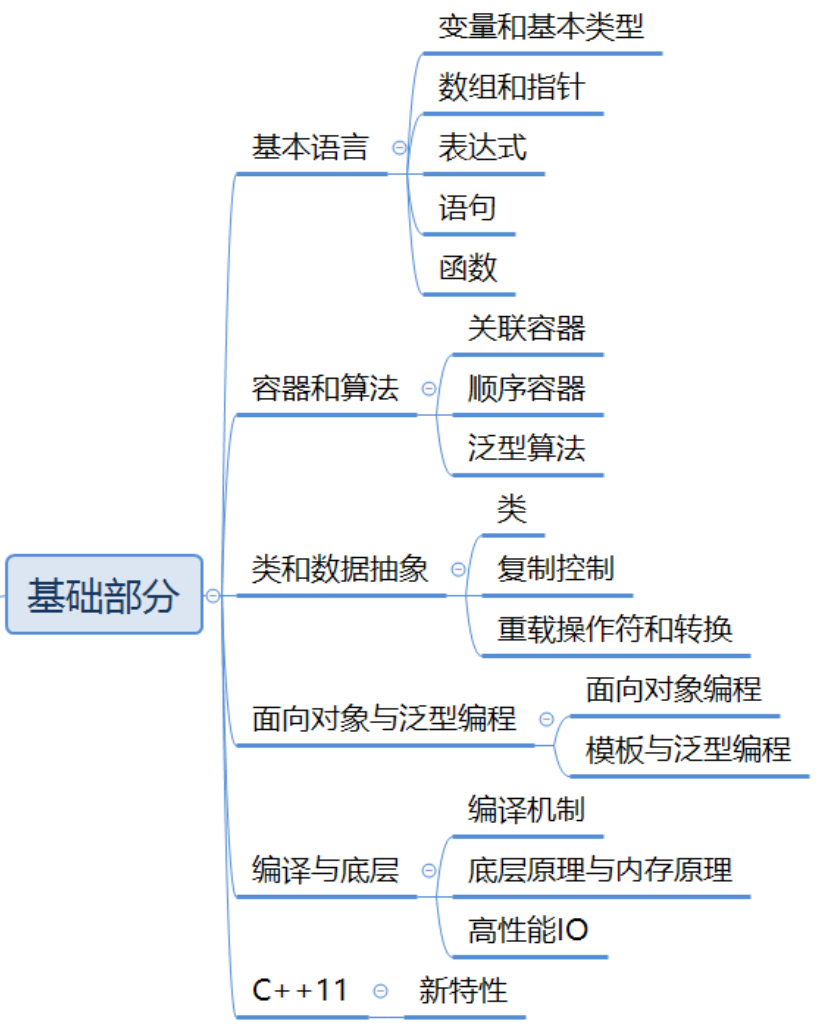
\includegraphics[width=0.5\columnwidth]{pic/overview.png}
	\caption{基础部分学习总览}
	\label{fig:overview}
	% \vspace{-5pt}
\end{figure}

\section{基本语言知识点}
C++语言同时支持五种编程风格:C风格(面向过程)、基于对象、面向对象、泛型和函数式。
在C++11之前抽象存在若干的缺陷,最严重的是缺少自动内存管理和对象级别的消息发送机制。
现代C++语言可以看作是三部分组成的:1.低级语言,大部分继承自C;2.现代高级语言特性,允许我们定义自己的类型以及组织大规模程序和系统;3.标准库,利用高级特性来提供有用的数据结构和算法。

\begin{itemize}
	\item \underline{static}关键字:在全局变量前面的时候,定义一个全局静态变量,在静态存储区,整个程序运行期间一直存在,未被初始化的全局静态变量将自动初始化为0,作用域在声明他的文件之外不可见。相对应的,局部静态变量,大体与全局静态变量是一样的,只是作用域只停留在局部,当方法退出时,全局静态变量不销毁而是继续驻留在静态存储区,直到方法被再次调用。
	\item 
\end{itemize}
